%% Ejemplo de la plantilla de latex para las diapositivas del Máster en IA 

%%%%%%%%%%%%%%%%%%%%%%%%%%%%
%% Valores para el ratio de aspecto: 43, 169 
%\documentclass[10pt, envcountsect, presentation, aspectratio=1610, hyperref={hypertexnames=true}]{beamer}
\documentclass[10pt, envcountsect, handout, aspectratio=1610, hyperref={hypertexnames=true}]{beamer}

%%%%%%%%%%%%%%%%%%%%%%%%%%%%

%%%%%%%%%%%%%%%%%%%%%%%%%%%%
%% Incluir fichero de estilo del máster
\input ../style/plantillaMasterIA.sty
%%%%%%%%%%%%%%%%%%%%%%%%%%%%

\addbibresource{../references.bib}



%\setbeameroption{show only notes} % Only notes
%\setbeameroption{show notes on second screen=right}  % Both
%\setbeamertemplate{note page}[compress]
\setbeameroption{hide notes} % Only slides


\renewcommand*\footnoterule{}
\setbeamerfont{footnote}{size=\tiny}




%\input{embed_video.tex}
%\usepackage{movie15}b
\usepackage{multimedia}


%%%%%%%%%%%%%%%%%%%%%%%%%%%%
%% Información que aparecerá en la portada
\title[Aprendizaje por Refuerzo]{Aprendizaje por Refuerzo}
\subtitle{Predicción On Policy con Aproximaciones} % short title for footer

\author[L. D. Hernández] % Para el pie de página, poner los autores abreviados separados por comas.
{%
	\sc{Luis Daniel Hernández Molinero }\\ % Autor 1
	\textit{Ciencia de la Computación e Inteligencia Artificial}\\  % Area de conocimiento
	\textit{Dept. Ingeniería de la Información y las Comunicaciones}\\  % Departamento
	\\   % No dejes espacio entre esta línea y la llave siguiente 
}

\institute[DIIC]% % Poner las iniciales de los diferentes departamentos de los autores separadas por comas.
{
	\textit{Universidad de Murcia}
}


\newcounter{lastyear}
\setcounter{lastyear}{\the\year}
\addtocounter{lastyear}{-1}

\date{\arabic{lastyear} / \the\year} % Curso académico


%%%%%%%%%%%%%%%%%%%%%%%%%%%%%%%%%%
%% Contenido de las diapositivas
\setbeamerfont{normal text}{size=\normalsize} % Modifica el tamaño del texto de las diapositivas.
\AtBeginDocument{\usebeamerfont{normal text}}

%%%%%%%%%%%%%%%%%%%%%%%%%%%%%%%%%%

\begin{document}	

%%%%%%%%%%%%%%%%%%%%%%%%%%%%%%%%%%




%%%%%%%%%%%%%%%%%%%%%%%%%%%%%%%%%%

\begin{frame}[plain]
	\titlepage
\end{frame}

%%%%%%%%%%%%%%%%%%%%%%%%%%%%%%%%%%

\begin{frame}{Índice de Contenidos}
	\tableofcontents 
	
\note{

}

\end{frame}










%%%%%%%%%%%%%%%%%%%%%%%%%%%%%%%%%%
%%%%%%%%%%%%%%%%%%%%%%%%%%%%%%%%%%
\section{Introducción}
%%%%%%%%%%%%%%%%%%%%%%%%%%%%%%%%%%
%%%%%%%%%%%%%%%%%%%%%%%%%%%%%%%%%%



\begin{frame}{Introducción}{Escalabilidad, generalización y flexibilidad a cambio de garantías teóricas}
\begin{itemize}
    \item La función de valor aproximada se representa \textbf{no como una tabla} sino como una \key{forma funcional parametrizada} con un vector de pesos $\mathbf{w} \in \mathbb{R}^d$.
    
    \item Escribiremos $\hat{v}(s, \mathbf{w}) \approx v_\pi(s)$ para \key{el valor aproximado del estado} $s$ dado el vector de pesos $\mathbf{w}$.
    
    \item Por ejemplo, $\hat{v}$ puede ser:
    \begin{itemize}
        \item Una \key{función lineal} \textbf{en las características del estado}, $[f_1(s), f_2(s), \ldots, f_d(s)]$, con $\mathbf{w}$ como el vector de pesos de las características.
        
        \item La función calculada por una \key{red neuronal artificial multi-capa}, con $\mathbf{w}$ como el vector de pesos de conexión en todas las capas.
        
        \item La función computada por un \key{árbol de decisión}, donde $\mathbf{w}$ son todos los números que definen los puntos de división y los valores de las hojas del árbol.
    \end{itemize}
    
    \item Típicamente, la \key{dimensionalidad} de $\mathbf{w}$ es mucho menor que el número de estados ($d \ll |S|$), y cambiar un peso afecta el valor estimado de muchos estados. \\ \hfil P.e. Go: $10^{600}$ secuencias para llegar a una de las $10^{170}$ combinaciones.
    
    \item Cuando se actualiza un solo estado, el \textbf{cambio} \key{se generaliza} desde ese estado para afectar los valores de muchos otros estados.
    
    \item Tal generalización hace que el \key{aprendizaje} sea potencialmente \textbf{más poderoso}, pero también potencialmente \textbf{más difícil de gestionar y entender}.
    
    \item Extender el aprendizaje por refuerzo a la aproximación de funciones también lo hace \key{aplicable a problemas parcialmente observables}, en los cuales el estado completo no está disponible para el agente.
    
\end{itemize}

\end{frame}




%%%%%%%%%%%%%%%%%%%%%%%%%%%%%%%%%%
%%%%%%%%%%%%%%%%%%%%%%%%%%%%%%%%%%
\section{Aproximación de Funciones de Valor}
	
	
%%%%%%%%%%%%%%%%%%%%%%%%%%%%%%%%%%
%%%%%%%%%%%%%%%%%%%%%%%%%%%%%%%%%%
\begin{frame}{Aproximación de Funciones de Valor}
\begin{itemize}
    \item Nos referimos a una \key{actualización individual} mediante la notación $s \mapsto u$, donde $s$ es el estado actualizado y $u$ es el objetivo de actualización hacia el cual se desplaza el valor estimado de $s$.
    \begin{itemize}
    	\item La  actualización de programación dinámica es \( S_t \mapsto \mathbb{E}^\pi[R_{t+1} + \gamma \hat{v}(S_{t+1}, \mathbf{w}_t) | S_t = s] \),
        \item La actualización Monte Carlo para la predicción de valor es $S_t \mapsto G_t$.
        \item La actualización TD(0) es \( S_t \mapsto R_{t+1} + \gamma \hat{v}(S_{t+1}, w_t) \)
        \item La actualización TD de n-pasos es $S_t \mapsto G_{t:t+n}$.
    \end{itemize}
    \item Es natural \key{interpretar cada actualización como un ejemplo} del comportamiento deseado de entrada-salida de la función de valor.
    \begin{itemize}
        \item \key{Hasta ahora}, la actualización  para \textbf{el valor estimado} de \( s \) simplemente \textbf{se desplaza una fracción} hacia el valor objetivo \( u \), manteniendo los demás valores estimados de los demás estados sin cambios.
        
        \item \key{Ahora}, la actualización $s \mapsto u$ significa que \textbf{el valor estimado} para el estado $s$ \key{debería ser lo más parecido} al valor objetivo $u$. Además, la actualización en \( s \) se generaliza de manera que los valores estimados de muchos otros estados también se cambiarán.
    \end{itemize}
    
    \item \key{Aprendizaje supervisado} Los métodos de aprendizaje automático que aprenden a imitar ejemplos de entrada-salida
    
    	\begin{itemize}
    		\item Cuando las salidas son números, como \( u \), el proceso a menudo se llama \textbf{aproximación de funciones}
    	\end{itemize}
    
    \item Utilizamos métodos de \key{aproximación de funciones} para la predicción de valor pasando a ellos el $s \mapsto u$ de cada actualización \textbf{como un ejemplo de entrenamiento}.
\end{itemize}
	
\end{frame}


%%%%%%%%%%%%%%%%%%%%%%%%%%%%%%%%%%
%%%%%%%%%%%%%%%%%%%%%%%%%%%%%%%%%%
\begin{frame}{Aproximación de Funciones de Valor: Restricciones}
	

\scalebox{1.2}{
\begin{minipage}{0.8\textwidth}
	\begin{itemize}
    \item En el aprendizaje por refuerzo es importante que  \key{el aprendizaje debe ser on-line} mientras el agente interactúa con su entorno o con un modelo de su entorno.
    
    \begin{itemize}
        \item Los métodos necesitan aprender eficientemente \textbf{a partir de datos adquiridos incrementalmente}.
    \end{itemize}
    
        
    ~
    
   
    \item El aprendizaje por refuerzo generalmente requiere métodos de aproximación de funciones capaces de manejar  \key{funciones objetivo no estacionarias}.

    \begin{itemize}
        \item En métodos de control basados en GPI a menudo buscamos aprender $q_\pi$ mientras $\pi$ cambia.
        
        \item Incluso si la política permanece igual, \textbf{los valores objetivo de los ejemplos de entrenamiento son no estacionarios} si son generados mediante \textit{métodos de refuerzo} (DP y TD learning).
    \end{itemize}
\end{itemize}
\end{minipage}}
\end{frame}



%%%%%%%%%%%%%%%%%%%%%%%%%%%%%%%%%%
%%%%%%%%%%%%%%%%%%%%%%%%%%%%%%%%%


\section{El Objetivo de Predicción}

\begin{frame}{El Objetivo de Predicción ($\overline{\text{VE}}$)}
	
\begin{itemize}
	\item \key{Medida de desempeño:} evaluar la calidad de las predicciones realizadas por un modelo.
	
	\item En el \key{caso tabular} \textbf{no era necesaria} una medida de desempeño (dependencia temporal).
	
	\begin{itemize}
	\item  \textbf{Por ejemplo}, la actualización de forma local:$V(s) \leftarrow V(s) + \alpha [Target - V(s)]$
	\end{itemize}
	
	\item En el \key{caso aproximado} \textbf{\underline{sí} es necesaria} una medida de desempeño (dependencia estrutural)
	
		\begin{itemize}
		\item  \textbf{Por ejemplo}, si modelamos los valores con una función lineal:  
				$
				V_\theta(s) = \theta_1 x_1 + \theta_2 x_2
				$ 
		\end{itemize}
	
	 

	
    \item Definimos el \key{Error Cuadrático Medio de Valor}, denotado $\overline{VE}$, como la \key[reddark]{función objetivo a minimizar}.
    \[
        \overline{\text{VE}}(\mathbf{w}) \doteq \sum_{s \in S} \mu(s) \left[ v_\pi(s) - \hat{v}(s, \mathbf{w}) \right]^2
    \]
    \item Especificamos una \key{distribución de estados} $\mu(s)$ con $\mu(s) > 0, \sum \mu(s) = 1$, representando cuánto nos importa el error en cada estado $s$.
    
    \item Bajo entrenamiento on-policy \key{a $\mu(s)$ se le llama la distribución on-policy}.
    
   \begin{itemize}
   	 \item En tareas episódicas, $\mu(s)$ se elige como la \textbf{fracción del tiempo} que se ha pasado en $s$.

    \item En tareas infinitas, la distribución en política $\mu(s)$ es la \textbf{distribución estacionaria} bajo $\pi$.
   \end{itemize}
\end{itemize}

\end{frame}


%%%%%%%%%%%%%%%%%%%%%%%%%%%%%%%%%%
%%%%%%%%%%%%%%%%%%%%%%%%%%%%%%%%%

\begin{frame}{Cálculo de la Distribución on-policy}
	
	\begin{itemize}
		\item Queremos calcular \key{la distribución on-policy}.
		\item En una \key[reddark]{tarea episódica}, \textbf{la distribución on-policy}  \textit{depende} de cómo se eligen los \textit{estados iniciales} de los episodios.
		\item Sea $h(s)$ la probabilidad de que un episodio comience en el estado $s$, y sea $\eta(s)$ el \textit{número de pasos de tiempo pasados}, en promedio, en el estado $s$ en un solo episodio.
		\[
		\eta(s) = h(s) + \sum_{\bar{s}} \eta(\bar{s}) \sum_a \pi(a|\bar{s})p(s|\bar{s}, a), \quad \text{para todo } s \in S.
		\]
		\item La \textbf{distribución on-policy} es entonces la fracción de tiempo pasado en cada estado normalizada para sumar uno:
		\[
		\mu(s) = \frac{\eta(s)}{\sum_{s'} \eta(s')}, \quad \text{para todo } s \in S.
		\]
		
		\item En una \key[reddark]{tarea no episódica} (con trayectorias infinitas) en el caso discreto, $h(s)=0$
	\end{itemize}
\end{frame}


%%%%%%%%%%%%%%%%%%%%%%%%%%%%%%%%%%
%%%%%%%%%%%%%%%%%%%%%%%%%%%%%%%%%%
\begin{frame}{El Objetivo de Predicción ($\overline{\text{VE}}$)}{¿Se puede alcanzar siempre?}
	\begin{itemize}
		\item \key{Error Cuadrático Medio de Valor}, denotado $\overline{\text{VE}}$, es nuestra función objetivo.
		\[
		\overline{\text{VE}}(\mathbf{w}) \doteq \sum_{s \in S} \mu(s) \left[ v_\pi(s) - \hat{v}(s, \mathbf{w}) \right]^2
		\]
		
		\item Un \key{objetivo ideal} en términos de  $\overline{\text{VE}}$ sería encontrar un \textbf{óptimo global}.
		\begin{itemize}
			\item Un vector de pesos $\mathbf{w}^*$ tal que $\overline{\text{VE}}(\mathbf{w}^*) \leq \overline{\text{VE}}(\mathbf{w})$ para todo $\mathbf{w}$.
		\end{itemize}
		
		\item \key{¿Es posible alcanzar este objetivo?}
		\begin{itemize}
			 \item \textbf{A veces es posible} para aproximadores de \textbf{funciones simples}, como los lineales. 
			 \item \textbf{Rara vez es posible} para aproximadores de \textbf{funciones complejas}, como las RNA y los árboles de decisión.
		\end{itemize}
		
		\item Los \textit{aproximadores de funciones complejas} pueden buscar converger en su lugar a un \key{óptimo local}.
		\begin{itemize}
			\item Esta garantía es \textit{típicamente lo mejor} que se puede decir para aproximadores de funciones no lineales, y \textbf{a menudo es suficiente}.
			\item Sin embargo, \textbf{para muchos casos de interés en RL no hay garantía de convergencia} a un óptimo, ni siquiera dentro de una \textit{distancia acotada} de un óptimo.
			\item Algunos \textbf{métodos pueden incluso divergir}, con su $\overline{\text{VE}}$ acercándose al infinito en el límite.
		\end{itemize}
	\end{itemize}
\end{frame}


%%%%%%%%%%%%%%%%%%%%%%%%%%%%%%%%%%
%%%%%%%%%%%%%%%%%%%%%%%%%%%%%%%%%%
\section{Métodos de Gradiente Estocástico y Semi-gradiente}

%%%%%%%%%%%%%%%%%%%%%%%%%%%%%%%%%%
%%%%%%%%%%%%%%%%%%%%%%%%%%%%%%%%%%
\subsection{Métodos de Gradiente Estocástico}

%%%%%%%%%%%%%%%%%%%%%%%%%%%%%%%%%%
%%%%%%%%%%%%%%%%%%%%%%%%%%%%%%%%%%
\begin{frame}{Métodos del Descenso de Gradiente Estocástico}
	\begin{itemize}
		\item Métodos de \key{Descenso de Gradiente}: 
		\begin{itemize}
			\item $\mathbf{w}_{t+1} = \mathbf{w}_t - \alpha \nabla \overline{\text{VE}}(\mathbf{w}_n)$, \qquad con  $\ds \overline{\text{VE}}(\mathbf{w}) \doteq \sum_{s \in S} \mu(s) \left[ v_\pi(s) - \hat{v}(s, \mathbf{w}) \right]^2$
			
			
			\item El vector de pesos es un \textit{vector columna} con un número fijo de componentes reales: $\mathbf{w} = (w_1, w_2, \dots, w_d)^\top$.
			
			\item $\overline{\text{VE}}$ debe ser diferenciable.
			$\ds
				\nabla f(\mathbf{w}) \doteq \left( \frac{\partial f(\mathbf{w})}{\partial w_1}, \frac{\partial f(\mathbf{w})}{\partial w_2}, \ldots, \frac{\partial f(\mathbf{w})}{\partial w_d} \right)^\top. 
			$
			
			\item La distribución on-policy $\mu(s)$ \key{no se puede calcular}.
			
			\begin{itemize}
				\item La distribución $\mu(s)$ emerge como resultado de seguir la política $\pi(a|s)$ y las transiciones del entorno $p(s'|s, a)$.
				\item Cuando ejecutamos episodios de acuerdo a $\pi(a|s)$ y $p(s'|s,a)$, se genera una cadena de Markov.
				\item Los estados visitados durante la ejecución reflejan la distribución $\mu(s)$ de visitas esperadas.
			\end{itemize}
		\end{itemize}
			
		\item Una buena estrategia en este caso es \key{tratar de minimizar el error en los ejemplos observados}.
		
		\item Método del \key{Descenso de Gradiente Estocástico} (SGD, Sthocastic-Gradient Method)
			\begin{itemize}
				\item En cada paso, observamos un nuevo ejemplo $S_t \mapsto v_\pi(S_t)$
				\item Por ahora, 
				\item[]\qquad - Conocemos el \textbf{valor verdadero bajo la política $v_\pi(S_t)$}.
				\item[]\qquad - La función de valor aproximada $\hat{v}(s, \mathbf{w})$ es una \textbf{función diferenciable} respecto a $\mathbf{w}$ para todo $s \in S$.
				\item \key{Función de actualización:}\vskip-0.9cm
				\begin{align}
					\mathbf{w}_{t+1} &\doteq \mathbf{w}_t - \frac{\alpha}{2} \nabla \left[ v_\pi(S_t) - \hat{v}(S_t, \mathbf{w}_t) \right]^2 \tag{9.4} \\
					&\doteq \mathbf{w}_t + \alpha \left[ v_\pi(S_t) - \hat{v}(S_t, \mathbf{w}_t) \right] \nabla \hat{v}(S_t, \mathbf{w}_t), \tag{9.5}
				\end{align}
				
				\item[]\vskip-0.7cm
				
				\item \key{SGD converge} si $\alpha$ decrementa en el tiempo de acuerdo a las condiciones $\sum_n \alpha_n(a)=\infty$ y $\sum_n \alpha^2_n(a)<\infty$
			\end{itemize}
	\end{itemize}
\end{frame}



%%%%%%%%%%%%%%%%%%%%%%%%%%%%%%%%%%
%%%%%%%%%%%%%%%%%%%%%%%%%%%%%%%%%%

\begin{frame}{Descenso de Gradiente de Monte Carlo}
	\begin{itemize}
		\item Ahora consideramos \(S_t \mapsto U_t\), \key{no es el valor verdadero}, \(v_\pi(S_t)\)
			\begin{itemize}
				\item $U_t  \approx v_\pi(S_t) $ (es ruido)
				\item $U_t = R_{t+1} + \gamma \hat{v}(S_{t+1}, \mathbf{w}_t)$ (es  un objetivo bootstrap que usa $\hat{v}$)
			\end{itemize}
			
				
		\item Cambiamos la \key{Función de actualización} del \key[reddark]{Método del Descenso de Gradiente Estocástico} (SGD):
			\begin{equation}
				\mathbf{w}_{t+1} \doteq \mathbf{w}_t + \alpha \left[ U_t - \hat{v}(S_t, \mathbf{w}_t) \right] \nabla \hat{v}(S_t, \mathbf{w}_t). \tag{9.7}
			\end{equation}
			
		\item[] \vskip-1.15cm
		
		\item \key{Si $U_t$ es una estimación no sesgada}, es decir, si $\mathbb{E}[U_t | S_t] = v_\pi(S_t)$ para cada $t$, entonces $\mathbf{w}_t$ está \textbf{garantizado que convergerá a un óptimo local} bajo las condiciones usuales de  para $\alpha$ decreciente.
		
		\centerline{$
			\sum_{n=1}^{\infty} \alpha_n(a) = \infty \quad \text{y} \quad \sum_{n=1}^{\infty} \alpha_n^2 < \infty
			$}
			
~

		\item La \key{versión de descenso de gradiente de Monte Carlo} es el Descenso del Gradiente Estocástico que usa $U_t=G_t$ para la predicción de valores de estado y se \textbf{garantiza que encontrará una solución óptima local}.
		
			\begin{itemize}
				\item El \key{objetivo de Monte Carlo} $U_t = G_t$ es \textbf{por definición una estimación no sesgada} de $v_\pi(S_t)$.
				\item Exigue la condiciones de aproximación estocástica
				\item Usa la ecuación de actualización (9.7)
				\item \textbf{Convergerá a una aproximación óptima local} de $v_\pi(S_t)$
			\end{itemize}
	\end{itemize}
\end{frame}


%%%%%%%%%%%%%%%%%%%%%%%%%
%%%%%%%%%%%%%%%%%%%%%%%%%
\begin{frame}{Algoritmo del Gradiente (Estocástico) de Monte Carlo}
	
	\centerline{\includegraphics[width=\textwidth]{fig/alg_gradiente_mc}}
	
	
\note<1>{
	\begin{itemize}
		\item Como entrada tenemos política que queremos evaluar y una función $V$-gorro que sea diferenciable.
		\item Se establece un tamaño de paso $\alpha$ y se inicializan los $d$-pesos.
		
		\item Entonces  aplicamos montecarlos una y otra vez con los siguientes pasos
		
		\begin{itemize}
			\item Se genera un episodio desde el estado inicial hasta un estado terminal.
			\item Para cada estado del episodio calculamos El retorno del estado.
			\item Actualizamos la ecuación que hemos llamado (9.7)
		\end{itemize}
	\end{itemize}
	\fin
}	

\end{frame}


%%%%%%%%%%%%%%%%%%%%%%%%%%%%%%%%%%
%%%%%%%%%%%%%%%%%%%%%%%%%%%%%%%%%%

\subsection{Métodos de  Semi-gradiente}

%%%%%%%%%%%%%%%%%%%%%%%%%%%%%%%%%%
%%%%%%%%%%%%%%%%%%%%%%%%%%%%%%%%%%
\begin{frame}{Métodos de  Semi-gradiente}
	\begin{itemize}
		\item Tenemos que, si observamos un ejemplo $S_t \mapsto V_t$:
			\begin{itemize}
				\item Si $V_t=v_\pi(S_t)$, el método del descenso del gradiente converge a un mínimo.
				\item Si $V_t=U_t$ responde a una muestra de Monte Carlo, $G_t$, también converge.
				\item ¿Y si $V_t=U_t$ es un objetivo calculado por bootstraping? p.e. $U_t = R_{t+1} + \gamma \hat{v}(S_{t+1}, \mathbf{w}_t)$ (DT)
			\end{itemize}
			
		\item Si \key{el target $U_t$ es por bootstrap}, dependerán del valor actual de pesos  \(\mathbf{w}_t\).
			\begin{itemize}
				\item Retornos de \(n\)-pasos: \(U_t = G_{t:t+n} =  R_{t+1} + \gamma R_{t+2} + \dots + \gamma^{n-1} R_{t+n} + \gamma^n \hat{v}_{t+n-1}(S_{t+n}, \mathbf{w}_{t+n-1}))\)
				\item Programación Dinámica:  
				$U_t= \ds
				\sum_a \pi(a | S_t) \sum_{s', r} p(s', r | S_t, a)[r + \gamma \hat{v}(s', \mathbf{w}_t)],
				$
				
			\end{itemize}
			Entonces, $U_t$ estará \textbf{sesgado} y \textbf{no producirán un verdadero método de descenso de gradiente}.
		
		\item Los pasos clave desde (9.4) hasta (9.5) \key{depende de que el objetivo $U_t$ sea independiente} de $\mathbf{w}_t$.
		
		\item Los métodos \textit{bootstrap} \textbf{no generan}  ejemplos del \textbf{gradiente verdadero}, pero incluyen  una parte del gradiente \citep{Barnard1993}.
		
		\item Llamamos \key[reddark]{métodos de semi-gradiente}, a aquellos que \key{usan} la siguiente función de actualización del \textit{descenso del gradiente estocástico}, la (9.7), usando como objetivo \textit{$U_t$ un valor obtenido por bootstrap}.
		
		~
		
		\centerline{\large$
			\mathbf{w}_{t+1} \doteq \mathbf{w}_t + \alpha \left[ U_t(\mathbf{w}_t) - \hat{v}(S_t, \mathbf{w}_t) \right] \nabla \hat{v}(S_t, \mathbf{w}_t)
		$}
		
		~
		
		E.d. Cuando $U_t$ depende de unos pesos $\mathbf{w}$ que aparecen en el gradiente.
				
	\end{itemize}

\end{frame}


%%%%%%%%%%%%%%%%%%%%%%%%%%%%%%%%%%
%%%%%%%%%%%%%%%%%%%%%%%%%%%%%%%%%%

\begin{frame}{Métodos  Semi-gradiente TD(0)}
	\begin{itemize}
		\item Aunque los métodos de \textit{semi-gradiente} (bootstrap) no convergen tan robustamente como los métodos de gradiente, \textit{convergen de manera confiable} en casos importantes.
	\end{itemize}
	
	\centerline{\includegraphics[width=\textwidth]{fig/alg_semi_gradiente_td}}

\end{frame}





%%%%%%%%%%%%%%%%%%%%%%%%%%%%%%%%%%
%%%%%%%%%%%%%%%%%%%%%%%%%%%%%%%%%%

\begin{frame}{El Algoritmo TD de Semi-gradiente con $n$ Pasos}
	%	\begin{itemize}
		%	\item Aunque los métodos de \textit{semi-gradiente} (bootstrap) no convergen tan robustamente como los métodos de gradiente, \textit{convergen de manera confiable} en casos importantes.
		%	\end{itemize}
	
	\centerline{\includegraphics[width=.78\textwidth]{fig/alg_n_step_semi_gradient}}
	
	\TPMargin{0mm}%
	\begin{textblock}{8}(7.8, 7) \small
		
		\begin{tcolorbox}[colback=green!5!white, left=2mm,right=2mm,top=2mm,bottom=2mm,boxsep=0mm,
			toptitle=0.5mm,bottomtitle=0.5mm]\footnotesize
			$\ds
			\mathbf{w}_{t+n} \doteq \mathbf{w}_{t+n-1} + \alpha \left[ G_{t:t+n} - \hat{v}(S_t, \mathbf{w}_{t+n-1}) \right] \nabla \hat{v}(S_t, \mathbf{w}_{t+n-1}),
			$
			%donde el retorno de $n$ pasos se generaliza desde (7.1) a:
			
			$\ds
			G_{t:t+n} \doteq R_{t+1} + \gamma R_{t+2} + \dots + \gamma^{n-1} R_{t+n} + \gamma^n \hat{v}(S_{t+n}, \mathbf{w}_{t+n-1}).
			$
		\end{tcolorbox}
	\end{textblock}
\end{frame}



%%%%%%%%%%%%%%%%%%%%%%%%%%%%%%%%%%%%%%%%%%%%%%%%%%%%%%%%%%%%%%%%%%%%
%%%%%%%%%%%%%%%%%%%%%%%%%%%%%%%%%%%%%%%%%%%%%%%%%%%%%%%%%%%%%%%%%%%%
\section{Métodos Lineales}

%%%%%%%%%%%%%%%%%%%%%%%%%%%%%%%%%%
%%%%%%%%%%%%%%%%%%%%%%%%%%%%%%%%%%
\begin{frame}{Métodos Lineales}
	\begin{itemize}
		\item $\hat{v}(\cdot, \mathbf{w})$ es una \key{función lineal} del vector de pesos $w$.
		
		\item Correspondiendo a cada estado $s$, hay un vector de valores reales $\mathbf{x}(s)$ con \textbf{el mismo número de componentes} que $\mathbf{w}$: $ \mathbf{x}(s) \doteq (x_1(s), x_2(s), \dots, x_d(s))^\top $, $ \mathbf{w} \doteq (w_1, w_2, \dots, w_d)^\top $
		
		\item Los\textbf{ métodos lineale}s aproximan la función de valor-estado mediante el \key{producto interno} entre $w$ y $x(s)$:
		
		\centerline{\large$\ds \hat{v}(s, \mathbf{w}) \doteq \mathbf{w}^T \mathbf{x}(s) = \sum_{i=1}^{d} w_i x_i(s).$}
		
		\item El vector $\mathbf{x}(s)$ se llama \key{vector de características} que representa el estado $s$.
		\begin{itemize}
			\item Cada componente $x_i(s)$ de $\mathbf{x}(s)$ es el valor de una función $x_i : \mathcal{S} \to \mathbb{R}$.
		
			\item Para métodos lineales, \textbf{las características son funciones base} para el \textit{conjunto de funciones aproximadas}.
				\begin{itemize}
					\item Se verá algún ejemplo posteriormente.
				\end{itemize}
		\end{itemize}

	\item \key{El gradiente} de la función de valor aproximada con respecto a $w$ en este caso es:
	{\large$\ds
	\nabla \hat{v}(s, \mathbf{w}) = \mathbf{x}(s)
	$}
	
	\item Así, en el caso lineal, \key{la actualización SGD} general (9.7) se reduce a una forma particularmente simple:
	\centerline{\large$
	\mathbf{w}_{t+1} \doteq \mathbf{w}_t + \alpha \left[ U_t - \hat{v}(S_t, \mathbf{w}_t) \right] \mathbf{x}(S_t).
	$}
	
	\item \key{El caso SGD lineal} es uno de los más favorables para el análisis matemático.
	\begin{itemize}
		\item Los \textit{resultados de convergencia} útiles para sistemas de aprendizaje suelen ser \textit{para métodos de aproximación de funciones lineales (o más simples)}.
		\item \textbf{En el caso lineal, solo hay un óptimo.}
	\end{itemize}
	\end{itemize}
	
\end{frame}


%%%%%%%%%%%%%%%%%%%%%%%%%%%%%%%%%%%%%%%%%%%%%%%%%%%%%%%%%%%%%%%%%
%%%%%%%%%%%%%%%%%%%%%%%%%%%%%%%%%%%%%%%%%%%%%%%%%%%%%%%%%%%%%%%%%

\subsection{\S Convergencia de los Métodos Lineales}

%%%%%%%%%%%%%%%%%%%%%%%%%%%%%%%%%%
%%%%%%%%%%%%%%%%%%%%%%%%%%%%%%%%%%
\begin{frame}{\S Convergencia de los Métodos Lineales}{Porque los estados se actualizan de acuerdo a la distribución on-policy.}
	\begin{itemize}
		\item El algoritmo \key{Monte Carlo con gradiente} converge al \textbf{óptimo global} del \textbf{VE} bajo aproximación lineal de funciones si $\alpha$ se reduce con el tiempo de acuerdo con las condiciones habituales.
	
		\item El algoritmo \key{TD(0) con semi-gradiente} \textbf{también converge} bajo aproximación lineal de funciones.
		\begin{itemize}
			\item Esto no se deduce de resultados generales sobre el descenso estocástico de gradiente (SGD).
			\item El vector de pesos \textit{converge a un punto cercano al óptimo local}.
		\end{itemize}
	
		\item Para el \key{caso continuo}, la actualización en cada tiempo $t$ para el algoritmo de semi-gradiente TD(0) es:
		\centerline{\large$
		\mathbf{w}_{t+1} \doteq \mathbf{w}_t + \alpha \left[ R_{t+1} + \gamma \mathbf{w}_t^T \mathbf{x}_{t+1} - \mathbf{w}_t^T \mathbf{x}_t \right] \mathbf{x}_t 
		$}
	
		\item Una vez que el sistema ha alcanzado el \textbf{estado estable}, para cualquier $\mathbf{w}_t$, el vector de pesos esperado puede escribirse como:
		
		\centerline{\large $
		\mathbb{E}[\mathbf{w}_{t+1} | \mathbf{w}_t ] = \mathbf{w}_t + \alpha \left( \mathbf{b} - \mathbf{A} \mathbf{w}_t \right)
		$} donde
		
		\centerline{ 
		$\mathbf{b} \doteq \mathbb{E}[R_{t+1}\mathbf{x}_t] \in \mathbb{R}^d, \quad \mathbf{A} \doteq \mathbb{E}\left[\mathbf{x}_t(\mathbf{x}_t - \gamma \mathbf{x}_{t+1})^T\right] \in \mathbb{R}^{d \times d} 
		$}
		
		\item Si el semi-gradiente TD(0) \textbf{converge}, debe converger al \textbf{punto fijo TD} del vector de pesos $\mathbf{w}_{TD}$:
		
			\centerline{ 
				$\mathbf{b} - \mathbf{A}\mathbf{w}_{TD} = 0 \quad
					\Rightarrow \quad
					\mathbf{b} = \mathbf{A}\mathbf{w}_{TD} \quad
					\Rightarrow \quad
					\mathbf{w}_{TD} \doteq \mathbf{A}^{-1}\mathbf{b} 
				$}
	
		\item En el \textbf{punto fijo TD}, también se ha demostrado (en el caso continuo) que el \textbf{VE} está dentro de una expansión acotada del error más bajo posible:
		$\ds
		\sqrt{VE(\mathbf{w}_{TD})} \leq \frac{1}{1-\gamma} \min_{\mathbf{w}} VE(\mathbf{w}).
		$
	\end{itemize}

	
	
\end{frame}


%%%%%%%%%%%%%%%%%%%%%%%%%%%%%%%%%%%%%%%%%%%%%%%%%%%%%%%%%%%%%%%%%
%%%%%%%%%%%%%%%%%%%%%%%%%%%%%%%%%%%%%%%%%%%%%%%%%%%%%%%%%%%%%%%%%

\subsection{Construcción de Características para Métodos Lineales}


%%%%%%%%%%%%%%%%%%%%%%%%%%%%%%%%%%%%%%%
%%%%%%%%%%%%%%%%%%%%%%%%%%%%%%%%%%%%%%%

\begin{frame}{Construcción de Características para Métodos Lineales}
	
	
	\begin{itemize}
		\item El \key{éxito} de los métodos lineales (\textit{LM}) \key{depende} críticamente de \textbf{cómo se representa los estados  en términos de características}.
		
		\item \textbf{Elegir características} apropiadas para la tarea es una forma importante de \key{añadir conocimiento previo del dominio} a los sistemas de aprendizaje por refuerzo.
		\begin{itemize}
			\item Intuitivamente, las características deben corresponder a los aspectos del espacio de estados a lo largo de los cuales la generalización puede ser apropiada.
		\end{itemize}
		
		\item Una \key{limitación} de la forma lineal es que \textit{no considera ninguna interacción entre características}
		\begin{itemize}
			\item Ejemplo: Se tienen dos atributos:
				\begin{itemize}
					\item \( s_1 = x_1(s)\): Si hay un obstáculo cerca (1 = no, 0 = si).  
					\item \( s_2 = x_2(s) \): Si el robot tiene un alto nivel de batería (1 = sí, 0 = no).  
	 
				
			\item Se considera un estabo bueno cuando no hay obstáculo cerca (\( s_1 = 1 \)) y hay suficiente batería (\( s_2 = 1 \)). Cualquier otro se considera malo.
			
			\item El modelo lineal $\hat{v}(s, \mathbf{w}) = w_1 s_1 + w_2 s_2$ 
%				\begin{itemize}
					\item[]\qquad  
					No captura la interacción entre \( s_1 \) y \( s_2 \).
%					\item[] \qquad
					simplemente suma las contribuciones de \( w_1 \) y \( w_2 \)
%				\end{itemize}  
		
						\end{itemize} 
		
		\end{itemize}
		
		\item Necesitamos modos de \textbf{definir características para combinaciones} de dos o más \key{dimensiones subyacentes del estado}.
		
	\end{itemize}
\end{frame}


%%%%%%%%%%%%%%%%%%%%%%%%%%%%%%%%%%%%%%%%%%%%%%%%%%%%%%%%%%%%%%%%%%%%%%%%%%%%%%%%
%%%%%%%%%%%%%%%%%%%%%%%%%%%%%%%%%%%%%%%%%%%%%%%%%%%%%%%%%%%%%%%%%%%%%%%%%%%%%%%%
\subsubsection{Polinomios}



%%%%%%%%%%%%%%%%%%%%%%%%%%%%%%%%%%%%%%%%%%%%%%%%
%%%%%%%%%%%%%%%%%%%%%%%%%%%%%%%%%%%%%%%%%%%%%%%%
\begin{frame}{Polinomios}
	
	\begin{itemize}
		\item Aunque las \key{características polinomiales básicas} que discutimos aquí \textit{no funcionan tan bien como otros tipos de características} en el aprendizaje por refuerzo, sirven como una buena introducción porque son simples y familiares.
		
		\item Supongamos un estado representativo $s$, con \textbf{dos componentes}, $\mathbf{x}(s) = (s_1, s_2)^T$,  $s_1 \in \mathbb{R}$ y $s_2 \in \mathbb{R}$.
			\begin{itemize}
				\item Si $s_1=s_2=0$ no quiero que la función valga 0 porque considero que es un estado objetivo deseable.

				\item Con solo  $(s_1, s_2)$ \key{no sería capaz de tener en cuenta ninguna interacción entre estas dimensiones}.
				
			\end{itemize}
		
		\item Se puede mejorar representando $s$ mediante el vector de características de cuatro dimensiones
			\begin{itemize}
				\item Con $\mathbf{x}(s) = (1, s_1, s_2, s_1 s_2)^T$ podemos construir la función 
				$\hat{v}(s, \mathbf{w}) = 1+  w_1 s_1 + w_2 s_2 + w_3 (s_1 \cdot s_2)$
				
					\begin{itemize}
						\item El término 1 evita que pares (0,0) se consideren indeseables.
						\item El nuevo término \(  (s_1 \cdot s_2) \) ajusta el valor solo cuando ambas características son 1
					
						\item Ahora el modelo puede asignar un valor más bajo a los estados malos.
					\end{itemize}
			\end{itemize}
	
		
		\begin{itemize}
			\item La característica inicial $1$ permite representar funciones afines en los números de estado originales, y la característica final, $s_1 s_2$, permite tener en cuenta \key{interacciones}.
		\end{itemize}
		
		\item Podemos usar vectores de características de dimensiones más altas.
			\begin{itemize}
				\item Ej: \(\mathbf{x}(s) = (1, s_1, s_2, s_1 s_2, s_1^2, s_2^2, s_1 s_2^2, s_1^2 s_2, s_1^2 s_2^2)^\top\)
			\end{itemize}
			
		\item En general, $\ds x_i(s) = s_i = \prod_{j=1}^k s_j^{c_{i,j}}$, $s_j\in\mathbb{R}$,  $c_{i,j} \in \{0, 1, \ldots, n\}$. En total $(n+1)^k$ características.
	\end{itemize}

\end{frame}


%%%%%%%%%%%%%%%%%%%%%%%%%%%%%%%%%%%%%%%%%%%%%%%%%%%%%%%%%%%%%%%%%%%%%%%%%%%%%%%%
%%%%%%%%%%%%%%%%%%%%%%%%%%%%%%%%%%%%%%%%%%%%%%%%%%%%%%%%%%%%%%%%%%%%%%%%%%%%%%%%
\subsubsection{Base de Fourier}



%%%%%%%%%%%%%%%%%%%%%%%%%%%%%%%%%%%%%%%%%%%%%%%%
%%%%%%%%%%%%%%%%%%%%%%%%%%%%%%%%%%%%%%%%%%%%%%%%

\begin{frame}{Base de Fourier}
	
	\begin{itemize}
		\item La \key{base de Fourie}r se utiliza \key{para aproximar una función objetivo} que \textbf{tiene patrones periódicos, suaves o continuos, o} cuando se necesita una representación eficiente para capturar \textbf{variaciones complejas}. 
		
		\begin{itemize}
			\item Su aplicación se basa en la descomposición de la función en una \key{combinación de senos y cosenos} con diferentes frecuencias.
		\end{itemize}
		
		\item Hay varios \key{motivos} para usar base de Fourier y la transformada de Fourier:
			\begin{itemize}
				\item La funciones es \textbf{periódicas}. \(f(x) = f(x + \tau)\) para todo \(x\) y algún período \(\tau\). 
				\item Funciones definidas en \textbf{intervalos acotados} (aperiódicas).
				\item Son funciones \textbf{suaves} o continuas (no necesariamente periódicas).
				\item Las funciones son \textbf{desconocidas} y deben ser aproximadas basándose en datos observados.
			\end{itemize}
		
		\item \key{Si se conoce la función a aproximar}:  
		\begin{itemize}
			\item Entonces, \textbf{los pesos de las funciones base se obtienen} mediante fórmulas simples y,  
			\item Con suficientes funciones base, esencialmente \textit{cualquier función puede ser aproximada} tan precisamente como se desee.  
		\end{itemize}
		
		\item \key{En RL}, donde las \textit{funciones a aproximar son desconocidas}, las funciones base de Fourier son de interés porque son \textit{fáciles de usar} y pueden funcionar bien en una variedad de problemas de RL.  

		
	\end{itemize}		
\end{frame}






%%%%%%%%%%%%%%%%%%%%%%%%%%%%%%%%%%
%%%%%%%%%%%%%%%%%%%%%%%%%%%%%%%%%%
\begin{frame}{Construcción de la Base}
	
	\begin{itemize}
		\item Las \key{funciones periódicas} $\tau$ se pueden aproximar por una \textbf{combinación lineal de funciones seno y coseno} que sean periódicas con período \(\tau\).  P.e. $cos\left(\frac{2\pi}{\tau} x\right)$ tiene periodo $\tau$.

		\item Si deseamos aproximar una \key{función aperiódica} definida sobre un intervalo acotado, podemos usar estas \textbf{funciones base - cosenos y bases - de Fourier} estableciendo:
		$
		\tau = \text{longitud del intervalo.}
		$

		
		\item Podemos usar \key{solo las funciones coseno}: Al establecer \(\tau\) como el \textbf{doble de la longitud del intervalo} de interés y restringirnos al \textbf{medio intervalo} \([0, \tau/2]\).  Esto es útil cuando la función es \textbf{par}:
			$
			f(-x) = f(x).
			$

		
		\item Alternativamente, es posible usar \key{solo funciones seno}, cuyas combinaciones lineales son siempre funciones \textbf{impares}:
		$
		f(-x) = -f(x)
		$.
		
		
		\item No excluye usar \textbf{ambas funciones seno y coseno} para aproximar sobre el intervalo \([0, \tau/2]\), lo que podría ser \textbf{ventajoso} en algunas circunstancias.
		
		\item \key{Construcción de la base:}
		
		\begin{itemize}
			\item  Cada estado es \(s = (s_1, s_2, \ldots, s_k)^\top\), con  \(s_i \in [0, 1]\)
			\item La \(i\)-ésima característica en la base coseno de Fourier de orden-\(n\) se escribi como $x_i(s) = \cos\left( \pi \mathbf{s}^\top \mathbf{c}_i \right)$, donde  \(\mathbf{c}_i = (c_{i1}, c_{i2}, \ldots, c_{ik})^\top\), con \(c_{ij} \in \{0, 1, \ldots, n\}\) para \(j = 1, \ldots, k\) y \(i = 1, \ldots, (n+1)^k\).
			\item Las características \textbf{pueden ser desplazadas y escaladas} para ajustarse al espacio de estados delimitado de una aplicación particular.
		\end{itemize}
		
		\item \key{Se sugiere} establecer el parámetro de tamaño de paso para la característica \(x_i\) como:
		$
		\alpha_i = \frac{\alpha}{\sqrt{c_{i1}^2 + \cdots + c_{ik}^2}},
		$
		excepto cuando cada \(c_{ij} = 0\), en cuyo caso \(\alpha_i = \alpha\).
		
	\end{itemize}		

\end{frame}





%%%%%%%%%%%%%%%%%%%%%%%%%%%%%%%%%%
%%%%%%%%%%%%%%%%%%%%%%%%%%%%%%%%%%
\begin{frame}{Base de Fourier para $n=3$ y $k=1$}
	\begin{itemize}
		\item El vector  \textbf{base de Fourier} son $(n+1)^k = (3+1)^1 = 4$ elementos para:  
		\begin{itemize}
			\item \textbf{Orden \( n = 3 \)} (máximo valor de frecuencia en cada dimensión).  
			\item \textbf{Dimensión \( k = 1 \)} (una variable: \( s_1 \) ).  
		\end{itemize}
	\end{itemize}

	\centerline{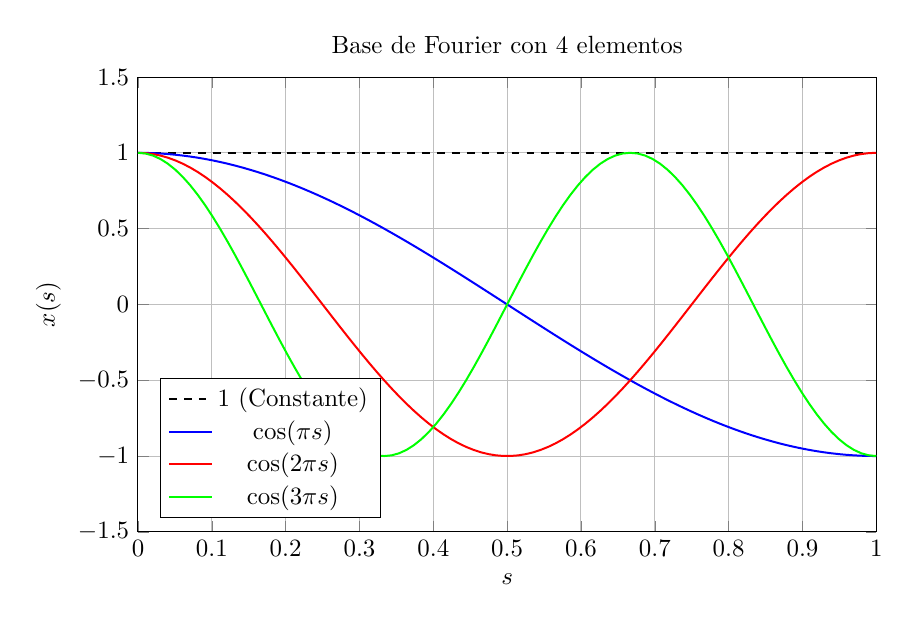
\begin{tikzpicture}[scale=.9]
		\begin{axis}[
			title={Base de Fourier con 4 elementos},
			xlabel={$s$}, ylabel={$x(s)$},
			xmin=0, xmax=1, ymin=-1.5, ymax=1.5,
			grid=major,
			legend pos=south west,
			width=12cm, height=8cm
			]
			% Gráfico 1: Constante
			\addplot[domain=0:1, samples=100, thick, dashed] {1};
			\addlegendentry{$1$ (Constante)}
			
			% Gráfico 2: cos(pi * s)
			\addplot[domain=0:1, samples=100, thick, blue] {cos(deg(pi*x))};
			\addlegendentry{$\cos(\pi s)$}
			
			% Gráfico 3: cos(2 * pi * s)
			\addplot[domain=0:1, samples=100, thick, red] {cos(deg(2*pi*x))};
			\addlegendentry{$\cos(2\pi s)$}
			
			% Gráfico 4: cos(3 * pi * s)
			\addplot[domain=0:1, samples=100, thick, green] {cos(deg(3*pi*x))};
			\addlegendentry{$\cos(3\pi s)$}
		\end{axis}
	\end{tikzpicture}}
\end{frame}




%%%%%%%%%%%%%%%%%%%%%%%%%%%%%%%%%%
%%%%%%%%%%%%%%%%%%%%%%%%%%%%%%%%%%
\begin{frame}{Bases de Fourier para  $k=1$}
	
	\includegraphics[width=\textwidth]{fig/fourier_series-011}

\end{frame}


%%%%%%%%%%%%%%%%%%%%%%%%%%%%%%%%%%
%%%%%%%%%%%%%%%%%%%%%%%%%%%%%%%%%%	
\begin{frame}{Base de Fourier para $n=3$ y $k=2$}
	
	\begin{itemize}
	\item Construimos la matriz  \textbf{base de Fourier} para:  
	\begin{itemize}
		\item \textbf{Orden \( n = 3 \)} (máximo valor de frecuencia en cada dimensión).  
		\item \textbf{Dimensión \( k = 2 \)} (dos variables: \( s_1 \) y \( s_2 \)).  
	\end{itemize}
	
	\item La matriz representará las combinaciones de frecuencias en las dos dimensiones (\( s_1 \) y \( s_2 \)) usando términos de la forma: $[
	\cos\left( \pi (c_1 s_1 + c_2 s_2) \right)
	$, 
	donde \( c_1, c_2 \) son los coeficientes de frecuencia en cada dimensión y varían entre \textbf{0 y 3} porque \( n = 3 \).  
	
	\vspace{0.3cm}
	
	\item La matriz está organizada como:
	\begin{enumerate}
		\item 1ª fila (\( c_2 = 0 \)): Frecuencias en \( s_1 \) (\( c_1 = 0, 1, 2, 3 \)).  
		\item 2ª fila (\( c_2 = 1 \)): Combinaciones cruzadas entre \( s_1 \) y \( s_2 \) con \( c_2 = 1 \).  
		\item 3ª fila (\( c_2 = 2 \)): Combinaciones cruzadas con \( c_2 = 2 \).  
		\item 4ª fila (\( c_2 = 3 \)): Combinaciones cruzadas con \( c_2 = 3 \).  
	\end{enumerate}
	
	\item \textbf{Número total de términos:} $(n+1)^k = (3+1)^2 = 16$
	
	\item Los 16 términos de la base son:
	\[
	\mathbf{x}(s) =
	\begin{bmatrix}
		1 & \cos(\pi s_1) & \cos(2\pi s_1) & \cos(3\pi s_1) \\
		\cos(\pi s_2) & \cos(\pi s_1 + \pi s_2) & \cos(\pi s_1 + 2\pi s_2) & \cos(\pi s_1 + 3\pi s_2) \\
		\cos(2\pi s_1) & \cos(2\pi s_1 + \pi s_2) & \cos(2\pi s_1 + 2\pi s_2) & \cos(2\pi s_1 + 3\pi s_2) \\
		\cos(3\pi s_1) & \cos(3\pi s_1 + \pi s_2) & \cos(3\pi s_1 + 2\pi s_2) & \cos(3\pi s_1 + 3\pi s_2)
	\end{bmatrix}.
	\]
	
		\item Para la actualización se proporcionan todas las filas consecutivas: un vector fila.
	\end{itemize}
	

	\TPMargin{0mm}%
\begin{textblock}{8}(10, 6)
%			DESCOMENTAR EL GRAFICO PARA QUE SALGA, ESTÁ COMENTADO PORQUE TARDA MUCHO EN PROCESAR EL FICHERO
	\scalebox{.6}{
			\begin{minipage}{\textwidth}
				\begin{tabular}{ccc}
					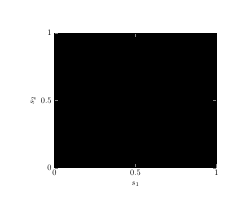
\begin{tikzpicture}[scale=0.3]
							\begin{axis}[view={0}{90}, colormap/blackwhite,
									xlabel={$s_1$}, ylabel={$s_2$},
									xtick={0, 0.5, 1}, ytick={0, 0.5, 1}]
									\addplot3[surf, samples=30, domain=0:1, y domain=0:1] {1};
								\end{axis}
						\end{tikzpicture} &  
					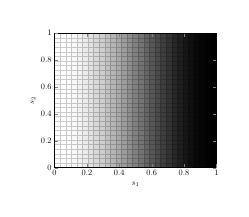
\begin{tikzpicture}[scale=.3]
							\begin{axis}[view={0}{90}, colormap/blackwhite,
									xlabel={$s_1$}, ylabel={$s_2$}]
									\addplot3[surf, samples=30, domain=0:1, y domain=0:1]
									{cos(deg(pi*x))};
								\end{axis}
							\end{tikzpicture} &  
					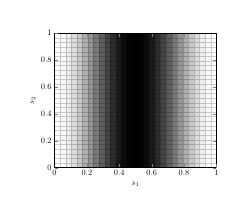
\begin{tikzpicture}[scale=.3]
							\begin{axis}[view={0}{90}, colormap/blackwhite,
									xlabel={$s_1$}, ylabel={$s_2$}]
									\addplot3[surf, samples=30, domain=0:1, y domain=0:1]
									{cos(deg(2*pi*x))};
								\end{axis}
						\end{tikzpicture} \\
			
					{$1$ (Constante)} & {$\cos(\pi s_1)$}  & {$\cos(2\pi s_1)$} \\
					&  &  \\
					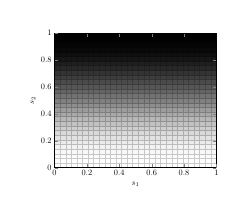
\begin{tikzpicture}[scale=.3]
						\begin{axis}[view={0}{90}, colormap/blackwhite,
								xlabel={$s_1$}, ylabel={$s_2$}]
								\addplot3[surf, samples=30, domain=0:1, y domain=0:1]
								{cos(deg(pi*y))};
							\end{axis}
						\end{tikzpicture} &
					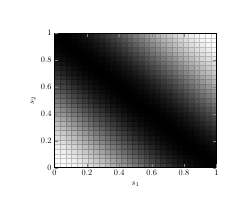
\begin{tikzpicture}[scale=.3]
							\begin{axis}[view={0}{90}, colormap/blackwhite,
									xlabel={$s_1$}, ylabel={$s_2$}]
									\addplot3[surf, samples=30, domain=0:1, y domain=0:1]
									{cos(deg(pi*x + pi*y))};
								\end{axis}
						\end{tikzpicture} & 
					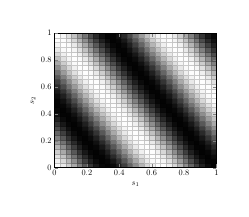
\begin{tikzpicture}[scale=.3]
							\begin{axis}[view={0}{90}, colormap/blackwhite,
									xlabel={$s_1$}, ylabel={$s_2$}]
									\addplot3[surf, samples=30, domain=0:1, y domain=0:1]
									{cos(deg(3*pi*x + 2*pi*y))};
								\end{axis}
						\end{tikzpicture} \\
					{$\cos(\pi s_2)$} &  {$\cos(\pi s_1 + \pi s_2)$}&  		{$\cos(3\pi s_1 + 2\pi s_2)$}\\
				\end{tabular}
			\end{minipage}}
\end{textblock}

\end{frame}
	




%%%%%%%%%%%%%%%%%%%%%%%%%%%%%%%%%%%%%%%%%%%%%%%%%%%%%%%%%%%%%%%%%%%%
%%%%%%%%%%%%%%%%%%%%%%%%%%%%%%%%%%%%%%%%%%%%%%%%%%%%%%%%%%%%%%%%%%%%

\subsubsection{Codificación Gruesa}

%%%%%%%%%%%%%%%%%%%%%%%%%%%%%%%%%%
%%%%%%%%%%%%%%%%%%%%%%%%%%%%%%%%%%
\begin{frame}{Codificación Gruesa (Coarse Coding)}
	
	\begin{columns}
		\begin{column}{.73\textwidth}
			\begin{itemize}
				\item Consideremos una tarea en la que la representación natural del conjunto de estados es un \key{espacio continuo bidimensional}.
				\begin{itemize}
					\item Las características corresponden a círculos en el espacio de estados.
					\item Si el estado está dentro de un círculo, entonces la característica correspondiente tiene el valor 1 y se dice que está \textbf{presente}; de lo contrario, la característica es 0 y se dice que está \textbf{ausente}.
				\end{itemize}
			\end{itemize}
		\end{column}
		%
		\begin{column}{.2\textwidth}
			\includegraphics[width=\linewidth]{fig/fig_coarse_coding}
		\end{column}
	\end{columns}

	\begin{itemize}
		\item Este tipo de característica con valores \textbf{1-0} se llama una \key{característica binaria}.
		
		\item Representar un estado con características que se superponen de esta manera (aunque no necesitan ser círculos o binarias) se conoce como \key{codificación gruesa}.
		
		\item Suponiendo una aproximación de función lineal mediante descenso de gradiente, consideremos el \key{efecto del tamaño y la densidad} de los círculos.
			\begin{itemize}
				\item Cada círculo corresponde a un peso (una \textit{componente individual} de $w$) 
				
				\item Si entrenamos en un estado, un punto en el espacio, entonces  \key{los pesos de todos los círculos que intersectan ese estado se verán afectados}.
				
				\item P.e. Cuado se actualice los pesos para $s$ del gráfico, afectará a 3 pesos.
			\end{itemize}
			
		\item La función de valor aproximada solo sumará si $x_i\not=0$: \quad $\hat{v}(s, w) \doteq w^T x(s) \doteq \sum_{i=1}^{d} w_i x_i(s)$
	\end{itemize}

	
\end{frame}



%%%%%%%%%%%%%%%%%%%%%%%%%%%%%%%%%%
%%%%%%%%%%%%%%%%%%%%%%%%%%%%%%%%%%
\begin{frame}
	\frametitle{Ejemplo: Grado de Grueso en Codificación}
	\begin{itemize}
		\item Aproximación de función lineal basada en codificación gruesa para aprender una función de onda cuadrada.

		\item Con sólo \textbf{una dimensión}, las regiones son \textit{intervalos} en lugar de círculos.
		
		\item El aprendizaje se repitió con \textbf{tres tamaños diferentes de intervalos}: estrecho, medio y amplio.
		\begin{itemize}
			\item Los tres casos tenían la \textit{misma densidad de características}, alrededor de 50 en el rango de la función que se aprende.
		\end{itemize}
		\item Los ejemplos de entrenamiento se \textbf{generaron uniformemente al azar} sobre este rango.
	\end{itemize}

	
	\centerline{\includegraphics[width=.6\textwidth]{fig/fig_coarse_coding_example}}
	
\end{frame}
	




%%%%%%%%%%%%%%%%%%%%%%%%%%%%%%%%%%%%%%%%%%%%%%%%%%%%%%%%%%%%%%%%%%%%
%%%%%%%%%%%%%%%%%%%%%%%%%%%%%%%%%%%%%%%%%%%%%%%%%%%%%%%%%%%%%%%%%%%%

\subsubsection{Codificación por Teselados}

%%%%%%%%%%%%%%%%%%%%%%%%%%%%%%%%%%
%%%%%%%%%%%%%%%%%%%%%%%%%%%%%%%%%%
\begin{frame}{Codificación por Teselados  (Tile Coding)}
	\begin{itemize}
		\item\key{ Teselado:} una partición del espacio en teselas.
		\item\key{ Si solo se usa una partición,} solo generaliza a los estados que caen en teselas previamente entrenadas.
		\item \key{Se superponen} varios teselados (uno por característica) \key{y se desplazan} una freacción de la tesela.
		\item El vector de características \(\mathbf{x}(s)\) tendrá \key{una componente para cada tesela} en cada teselado.
		\item \textit{Ejemplo:}
	
		\centerline{\includegraphics[width=.8\linewidth]{fig/fig_tile_coding}}
	
			\begin{itemize}
				\item En este ejemplo, hay \(4 \times 4 \times 4 = 64\) componentes, todos los cuales serán 0 excepto los cuatro correspondientes a las 'tiles' en las que cae \(s\). 
			\end{itemize}
		\end{itemize}
	
\end{frame}




%%%%%%%%%%%%%%%%%%%%%%%%%%%%%%%%%%
%%%%%%%%%%%%%%%%%%%%%%%%%%%%%%%%%%
\begin{frame}{Codificación por Teselados  (Tile Coding)}
	\begin{itemize}
	\item Si el número, $n$, de características activas, cumple \(n \ll d\): Hay ventajas computacionales (solo sumas)
	
		\begin{itemize}
			\item \textit{Ejemplo:} Un espacio de estados dividido en 50 mosaicos/teselas. Un estado $s$ cumple
				$\mathbf{x}(s) = [1, 0, 1, 0, 0, \ldots , 0]$. 
				La aproximación de la función de valor \( \hat{v}(s) \) es $\hat{v}(s) = w_1 + w_3$
		\end{itemize}
	
		
	\item \key{La generalización} (capacidad del modelo para estimar valores de cualquier estado)\key{ se ve afectada} por:
	\end{itemize}
	
	\begin{columns}
		\begin{column}{.5\textwidth}
			\begin{itemize}
				\item[]
				\begin{itemize}
					\item \textbf{El desplazamiento:}
					
				\item[] Las teselaciones desplazadas asimétricamente, la generalización es más esférica y homogénea.
				\end{itemize}
			\end{itemize}
			
			\centerline{\includegraphics[width=.6\linewidth]{fig/fig_tile_coding_patterns}}
			
		\end{column}
		
		\begin{column}{.43\textwidth}
		
			\begin{itemize}
				\item[] 	
				\begin{itemize}
					\item  \textbf{El patrón:}
					
					\item[]  Las teselas cuadradas generalizan aproximadamente igual en cada dimensión. Las  alargadas en una dimensión. Si unos son más delgados discriminan más. Si en diagonal, generalizan a lo largo de la diagonal. También pueden ser irregulares (aunque raros en la práctica).
				\end{itemize}
			\end{itemize}
			
			\centerline{\includegraphics[width=.6\linewidth]{fig/fig_tile_shapes}}
			
			\vfill
			
			~
			
				
		\end{column}
	\end{columns}
	
	\begin{itemize}
		\item El número de teselados, tamaño de las teselas, desplazamiento, patrón, determinarán la resolución o finura de la aproximación asintótica.
	\end{itemize}
	
\end{frame}




%%%%%%%%%%%%%%%%%%%%%%%%%%%%%%%%%%%%%%%%%%%%%%%%%%%%%%%%%%%%%%%%%%%%
%%%%%%%%%%%%%%%%%%%%%%%%%%%%%%%%%%%%%%%%%%%%%%%%%%%%%%%%%%%%%%%%%%%%

\subsubsection{Funciones de Base Radial}



	

%%%%%%%%%%%%%%%%%%%%%%%%%%%%%%%%%%
%%%%%%%%%%%%%%%%%%%%%%%%%%%%%%%%%%
\begin{frame}{Funciones de Base Radial (RBF)}
	\begin{itemize}
		\item Las \key{funciones de base radial} \textbf{(RBFs)} son la \textit{generalización natural de la codificación gruesa} a \textit{características de valores continuos}.
		
		\item En lugar de que cada característica sea 0 o 1, \key{puede ser cualquier valor en el intervalo [0, 1]}, reflejando varios grados en los que la característica está presente.
		
		\item Una característica RBF típica, $x_i$, es la \key{respuesta \textit{Gaussiana}} $x_i(s)$ 
		\begin{equation*}
			x_i(s) = \exp\left(-\frac{\left\| s - c_i \right\|^2}{2\sigma_i^2}\right)
		\end{equation*}
		(De)crecimiento exponencial en función de la distancia de un estado a un prototipo de la característica en relación con el \textit{ancho} de la característica:
		\begin{itemize}
			\item	\(s\): Estado actual.  
			\item \(c_i\): Centro prototípico de la función base radial \(i\).  
			\item \(\sigma_i\): Parámetro de ancho, controla la dispersión o escala de la función.  
			\item $\left\| s - c_i \right\|$: Distancia Euclidiana entre el estado $s$ y el centro (se puede considerar otras). 
		\end{itemize}
		
		
		\centerline{\includegraphics[width=0.5\linewidth]{fig/fig_rbf_example} \quad \includegraphics[width=0.2\linewidth]{fig/fig_gaussinas2D}}
	\end{itemize}

\end{frame}
	

%%%%%%%%%%%%%%%%%%%%%%%%%%%%%%%%%%
%%%%%%%%%%%%%%%%%%%%%%%%%%%%%%%%%%
\begin{frame}{Más sobre Funciones de Base Radial (RBF)}
	\begin{itemize}

		\item \key{Campos de aplicación:} Redes neuronales, aprendizaje por refuerzo, métodos de aproximación funcional, clasificación, clustering, modelos de regresión, procesamiento de señales e imágenes, modelado de superficies y campos de potencial, control adaptativo, sistemas dinámicos, métodos de optimización, procesos Gaussianos y aprendizaje Bayesiano.
		
		\item Hay \key{varias funciones} de base radial:
		
		\begin{itemize}
			\item \textit{Gaussiana:} 
			$ \varphi(r) = \exp(-\gamma r^2) $
			\item \textit{Multicuadrática:} 
			$ \varphi(r) = \sqrt{1 + (\gamma r)^2} $
			\item \textit{Inversa cuadrática:} 
			$ \varphi(r) = \frac{1}{1 + (\gamma r)^2} $
			\item \textit{Inversa multicuadrática:} 
			$ \varphi(r) = \frac{1}{\sqrt{1 + (\gamma r)^2}} $
		\end{itemize}
		
		
		\hfil donde $ r = \left\| \mathbf{x} - \mathbf{c} \right\| $ y $\gamma > 0$ es un parámetro de escala.
		
		
		\item La \key{principal ventaja} de las RBFs sobre características binarias es que producen \textit{funciones aproximadas que varían suavemente y son diferenciables}.
		
		
		\item Aunque esto es atractivo, 
		\begin{itemize}
			\item en la mayoría de los casos \key{no tienen una importancia práctica significativa}.
		
			\item Todos estos métodos \key{requieren} una \textit{complejidad computacional adicional sustancial} (en comparación con la codificación gruesa) y con frecuencia \textit{reducen el rendimiento} cuando hay más de dos dimensiones de estado.
		\end{itemize}
		
	\end{itemize}

\end{frame}





%%%%%%%%%%%%%%%%%%%%%%%%%%%%%%%%%%%%%%%%%%%%%%%%%%%%%%%%%%%%%%%%%%%%
%%%%%%%%%%%%%%%%%%%%%%%%%%%%%%%%%%%%%%%%%%%%%%%%%%%%%%%%%%%%%%%%%%%%

\section{Métodos No Lineales}




%%%%%%%%%%%%%%%%%%%%%%%%%%%%%%%%%%
%%%%%%%%%%%%%%%%%%%%%%%%%%%%%%%%%%
\begin{frame}{Redes Neuronales Artificiales como Funciones no-Lineales}
	\begin{itemize}
		\item Las \key{redes neuronales artificiales} (\textbf{RNAs}) son ampliamente utilizadas para la aproximación de funciones no lineales.
		\item \key[reddark]{Propiedad de Aproximación Universal:} 
		\begin{itemize}
			\item\key{ Una RNA con una sola capa oculta} que contenga un número suficientemente grande de unidades sigmoides \key{puede aproximar cualquier función continua} en una región compacta del espacio de entrada de la red \key{con cualquier grado de precisión} \citep{cybenko1989approximation}.
			
			\begin{itemize}
				\item Esto también es cierto para otras funciones de activación no lineales que cumplen condiciones suaves, pero la no linealidad es esencial.
			\end{itemize}
		\end{itemize}
		
		
		
		\item El resultado de un nodo (neurona) : $\ds f\left(z\right)=f\left( \sum_{i=1}^{n} w_i x_i + b \right)$
		
		
		\begin{itemize}
		 \item Entradas: \( x_1, x_2, \ldots, x_n \)  
		  - Pesos asociados: \( w_1, w_2, \ldots, w_n \)  
		  - Sesgo (bias): \( b \)  
		  - Función de activación: \( f \)  
		\end{itemize}
	
		
		\item \key{Funciones de activación} para conseguir la no-linealidad.
		
			\begin{minipage}{.5\textwidth}
				\begin{itemize}					
					\item \textbf{Sigmoide:}  
					$\ds
					\sigma(x) = \frac{1}{1 + e^{-x}}
					$
					
					\item \textbf{Tangente Hiperbólica (Tanh):}  
					$\ds
					\tanh(x) = \frac{e^x - e^{-x}}{e^x + e^{-x}}
					$
					
					\item \textbf{ReLU (Rectified Linear Unit):}  
					$
					f(x) = \max(0, x)
					$
					
					\item \textbf{Softmax:}  
					$\ds
					\text{Softmax}(x_i) = \frac{e^{x_i}}{\sum_{j} e^{x_j}}
					$
				\end{itemize}
			\end{minipage}
			%
			\begin{minipage}{.4\textwidth}
				\begin{itemize}

					\item \textbf{Leaky ReLU:}  
					$
					f(x) = 
					\begin{cases} 
						x & \text{si } x > 0 \\
						\alpha x & \text{si } x \leq 0
					\end{cases}
					$
					donde \( \alpha \) es un valor pequeño (p.e, 0.01).
					
					\item \textbf{ELU (Exponential Linear Unit):}  
					$
					f(x) = 
					\begin{cases} 
						x & \text{si } x > 0 \\
						\alpha (e^x - 1) & \text{si } x \leq 0
					\end{cases}
					$
				\end{itemize}
			\end{minipage}

	\end{itemize}

\end{frame}







%%%%%%%%%%%%%%%%%%%%%%%%%%%%%%%%%%
%%%%%%%%%%%%%%%%%%%%%%%%%%%%%%%%%%
\begin{frame}{Qué Aportan las Redes Neuronales Artificiales en RL}
	
\begin{itemize}
	\item \key{Un ejemplo} de Red Neuronal Artificial \textit{Feedforward} (no recurrente):

	\begin{minipage}{.45\textwidth}
		\begin{tikzpicture}[scale=.8, > = {Latex[width=4pt,length=8pt]},  transform shape]
			
			\node (L0) at (0,1.75) {$H^{(0)}$};
				
			% Input Layer
			\node[circle,draw,label=left:$x_1$] (I1) at (0,1) {};
			\node[circle,draw,label=left:$x_2$] (I2) at (0,-1) {};
			
			
			\node (L1) at (2,1.75) {$H^{(1)}$};
			% Hidden Layer
			\node[circle,draw] (H1) at (2,1) {$h_1$};
			\node[circle,draw] (H2) at (2,-1) {$h_2$};
			
			% Output Layer
			\node (L1) at (4,1.75) {$H^{(2)}$};
			\node[circle,draw] (O) at (4,0) {};
			
			\node (OO) at (5,0) {$\hat{v}$};
			
			% Connections Input-Hidden
			\draw[->] (I1) -- node[above] {$w_{11}$} (H1);
			\draw[->] (I1) -- node[above left, pos=0.4, shift={(-0.2,0)}] {$w_{21}$} (H2);
			\draw[->] (I2) -- node[below left, pos=0.4, shift={(-0.2,0)} ] {$w_{12}$} (H1);
			\draw[->] (I2) -- node[below] {$w_{22}$} (H2);
			
			
			%node[above] {$\gamma R_2$} (S2);
			
			% Connections Hidden-Output
			\draw[->] (H1) -- node[above] {$w_{1}$} (O);
			\draw[->] (H2) -- node[below] {$w_{2}$} (O);
			
			\draw[->] (O) -- (OO);
			
		\end{tikzpicture}
	\end{minipage}
	%
	\begin{minipage}{.4\textwidth}
		\begin{itemize}
			\item Primera Capa (oculta)
				\begin{itemize}
					\item $h_1^{(1)}=f_1(w_{11} x_1 + w_{12} x_2 + b_1)$
					
					\item $h_2^{(1)}=f_2(w_{21} x_1 + w_{22} x_2 + b_2)$
				\end{itemize}
			
			\item Segunda Capa (salida)
				\begin{itemize}
					\item $\hat{v}=h^{(2)} = f(w_1 h_1 + w_2 h_2 + b)$
				\end{itemize}
			
		\end{itemize}
	\end{minipage}
	
	
	\item[]
	
	~
	
	\item[] 
	
	~

	\item \key{Entrenar las capas ocultas} de una RNA es una \key{forma de crear automáticamente características} apropiadas para un problema dado, permitiendo representaciones jerárquicas sin depender exclusivamente de características diseñadas manualmente.
		
	\item En Aprendizaje por Refuerzo (RL), \key{las RNAs se pueden usar para}
		
		\begin{itemize}
			\item \textbf{aprender} funciones de valor $V$ o $Q$ (en lo que estamos), 
			\item pueden \textbf{maximizar} la recompensa esperada (REINFORCE) 
			\item puede aplicarse en un algoritmo de \textbf{gradiente de políticas} (Actor-Crítico). 
		\end{itemize}
		
\end{itemize}
	
\end{frame}




%%%%%%%%%%%%%%%%%%%%%%%%%%%%%%%%%%
%%%%%%%%%%%%%%%%%%%%%%%%%%%%%%%%%%
\begin{frame}{Esto va de Derivadas Parciales}

\begin{itemize}
	\item \key{Recordemos} la actualización de los pesos para estimar $V$ por TD:
	\begin{equation*}
		\mathbf{w}_{t+1} \doteq \mathbf{w}_t + \alpha \left[\overbrace{ \underbrace{R_{t+1} + \gamma  \hat{v}(S_{t+1}, \mathbf{w}_t)}_{U_t}  - \hat{v}(S_t, \mathbf{w}_t) }^{Error} \right] \nabla \hat{v}(S_t, \mathbf{w}_t)
	\end{equation*}
	
	
	\item \key{Es necesario estimar} la \textbf{derivada parcial de una función objetivo con respecto a cada peso}, dados los valores actuales de todos los pesos de la red.
	
	\item \textbf{La forma más exitosa} de hacer esto en RNAs con capas ocultas es el  \key{algoritmo de retropropagación (backpropagation)}.
	
		\begin{itemize}
			\item Producir \textbf{buenos resultados} para redes poco profundas
			\item \textbf{Puede no funcionar bien} para RNAs  \textbf{con muchas capas profundas}
				\begin{itemize}
					\item Problemas de \key{sobreajuste}.
					\item El \textit{backpropagation} es extremadamente \key{lento}.
					\item Las \key{derivadas parciales} calculadas son casi \key{nulas} en las primeras capas.
				\end{itemize}
		\end{itemize}

	\item A pesar de todo, \textbf{un tipo de RNA profunda}, la \key{red convolucional profunda},   ha demostrado tener aplicaciones impresionantes de aprendizaje por refuerzo
		\begin{itemize}
			\item Compensa más las ventajas que los inconvenientes.
		\end{itemize}
\end{itemize}

\end{frame}






%%%%%%%%%%%%%%%%%%%%%%%%%%%%%%%%%%%%%%%%%%%%%%%%%%%%%%%%%%%%%%%%%%%%
%%%%%%%%%%%%%%%%%%%%%%%%%%%%%%%%%%%%%%%%%%%%%%%%%%%%%%%%%%%%%%%%%%%%

\section{Métodos No Paramétricos}


%%%%%%%%%%%%%%%%%%%%%%%%%%%%%%%%%%
%%%%%%%%%%%%%%%%%%%%%%%%%%%%%%%%%%
	\begin{frame}{Aproximación de Funciones Basada en Memoria}
		\begin{itemize}
			\item \key{Aprendizaje paramétrico:} $\hat{v}(s, \mathbf{w}) \approx v_\pi(s)$
				\begin{enumerate}
					\item Se genera una \textbf{actualización individual}, mediante la notación $S_t \mapsto U_t$,
					\item Usamos \textbf{Descenso del Gradiente Estocástico}: 
					$
					\mathbf{w}_{t+1} \doteq \mathbf{w}_t + \alpha \left[ U_t - \hat{v}(S_t, \mathbf{w}_t) \right] \nabla \hat{v}(S_t, \mathbf{w}_t)
					$
					\item \textbf{Tiramos la muestra} y volvemos a 1.
				\end{enumerate}
				
			\item[]	\key{Cuando se necesita un valor aproximado para un estado}  la función se evalúa en ese estado usando \textbf{los parámetros más recientes} producidos por el algoritmo de aprendizaje.
			

			~
				
			\item \key{Aprendizaje perezoso (Lazy learning):} Almacena un subconjunto de ejemplos de entrenamiento en memoria a medida que llegan, sin actualizar ningún parámetro.
			\begin{itemize}
				\item Siempre que se necesite una estimación del valor para un estado consultado, se recupera un \textbf{conjunto de ejemplos de la memoria, \( \mathcal{D} \),} y \textbf{se utiliza} para calcular una estimación del valor para el estado consultado.
			\end{itemize}
			
			\item Los métodos de aproximación de funciones basadas en memoria son \key{métodos no paramétricos}.
			\begin{itemize}
				\item La \textbf{forma de la función de aproximación no está limitada a una clase parametrizada fija} de funciones.
				\item La forma está \textbf{determinada por los propios ejemplos de entrenamiento}, que dependerá de cómo combinarlos.
			
				\item Se espera que a más ejemplos de entrenamiento en la memoria, se produzcan aproximaciones  más precisas para \textbf{cualquier función objetivo}.
				
			\end{itemize}
		\end{itemize}
	\end{frame}
	
%%%%%%%%%%%%%%%%%%%%%%%%%%%%%%%%%%
%%%%%%%%%%%%%%%%%%%%%%%%%%%%%%%%%%
\begin{frame}{Ejemplos de Aproximación Basada en Memoria }
	\begin{itemize}
		\item  \key{Vecino más cercano:}
			\begin{itemize}
				\item El estado de consulta es \(s\)
				\item \(s^* \rightarrow g\) es el ejemplo en memoria cuyo estado \(s^*\) es el más cercano a \(s\)
				\item Retornar $\hat{v}(s)=v(s^*)$
			\end{itemize}
			
		\item \key{k-vecinos más cercanos:} $\ds \hat{v}(s, \mathcal{D}) = \frac{\sum_{i \in \mathcal{N}(s)} w_i V(S_i)}{\sum_{i \in \mathcal{N}(s)} w_i}$
		\begin{itemize}
			\item \( \mathcal{N}(s) \): Conjunto de los \( k \) vecinos más cercanos al estado \( s \).  
			\item \( V(S_i) \): Valor almacenado para el vecino \( S_i \).  
			\item \( w_i \): Peso asignado al vecino \( S_i \), definido como: $w_i = \frac{1}{d(s, S_i) + \epsilon} $. \( d(s, S_i) \) es la distancia entre estados y  \( \epsilon  > 0\).
		\end{itemize}
		
		\item \key{Regresión con núcleos (Kernel regression):} Es un método basado en memoria que calcula un promedio ponderado mediante un núcleo de los objetivos de todos los ejemplos almacenados en memoria, asignando el resultado al estado consultado.
		$\ds \hat{v}(s, \mathcal{D}) = \sum_{s' \in \mathcal{D}} k(s, s') g(s')$.  \( g(s') \) denota el \textit{objetivo para el estado} \( s' \).
		
		\begin{columns}
			\begin{column}{.4\textwidth}
				\begin{itemize}
					\item \textit{Núcleo Lineal:}
					$
					k(s, s') = s^T s'
					$
					
					\item \textit{Núcleo Polinómico:}
					$
					k(s, s') = (s^T s' + c)^d
					$
					
					\item \textit{Núcleo Gaussiano (RBF - Radial Basis Function):}
					$
					k(s, s') = \exp\left(-\frac{\|s - s'\|^2}{2\sigma^2}\right)
					$
				\end{itemize}
			\end{column}
			%
			\begin{column}{.5\textwidth}
				\begin{itemize}
					\item \textit{Objetivo TD(0):}
					$\ds
					g(s') = r(s', a) + \gamma \hat{v}(s'')
					$
					
					\item \textit{Objetivo Monte Carlo:}
					$
					g(s') = G(s') = \sum_{t=0}^{T} \gamma^t r_t
					$
					
					\item \textit{Promedio Empírico (Offline):}
					$
					g(s') = \frac{1}{n} \sum_{i=1}^{n} r_i(s')
					$
					(Usa los valores observados en $\cal D$  para calcular el promedio de recompensas asociadas al estado)
				\end{itemize}
			\end{column}
		\end{columns}
		
	\end{itemize}
\end{frame}




%%%%%%%%%%%%%%%%%%%%%%%%%%%%%%%%%%
%%%%%%%%%%%%%%%%%%%%%%%%%%%%%%%%%%
% BIBLIOGRAFÍA
%%%%%%%%%%%%%%%%%%%%%%%%%%%%%%%%%%
%%%%%%%%%%%%%%%%%%%%%%%%%%%%%%%%%%


%%%%%%%%%%%%%%%%%%%%%%%%%%%%%%%%%%%%%%%%%%%%%%%%%%%%%%%%%%%%%%%%%%%%
%%%%%%%%%%%%%%%%%%%%%%%%%%%%%%%%%%%%%%%%%%%%%%%%%%%%%%%%%%%%%%%%%%%%

\section{Referencias}

% Redefinimos la apariencia
%\setbeamertemplate{headline}{}
%\setbeamertemplate{frametitle}{\vskip 0.5cm	\small{\textbf{\insertframetitle}}}
%\setbeamertemplate{footline}{}






% Mostramos la bibliografía
% \begin{frame}[allowframebreaks] %% Si ocupa más de una página
\begin{frame}{Referencias} %% Si hay sólo una página
	
%	\begin{frame}{Referencias} %% Si hay sólo una página
		\nocite{Sutton2018, silver2015, Hado2018Lecture3}
		
		% \vskip -5cm %% Para ajustar la distancia al comienzo	
		%\bibliography{references}	
		\printbibliography[heading=none]
	\end{frame}    
	
	
	
	%%%%%%%%%%%%%%%%%%%%%%%%%%%%%%%%%%
	%%%%%%%%%%%%%%%%%%%%%%%%%%%%%%%%%%
	


%%%%%%%%%%%%%%%%%%%%%%%%%%%%%%%%%%
%%%%%%%%%%%%%%%%%%%%%%%%%%%%%%%%%%


\end{document}



